% !TEX root = main.tex

%------------------------------------------------
%\newpage
%\chapter[Residues]{Evaluating Contour Integrals Using Residues}
\chapter{Evaluating Contour Integrals Using Residues}
\section{Motivation}
Let $\mathcal{C}$ be a simple, closed anticlockwise contour.  In the previous section we saw how certain integrals of the form
\[
\int_{\mathcal{C}} f
\]
may be calculated using Cauchy's Integral Formula, when $f$ is a function holomorphic on region $\mathcal{R} \backslash \set{z_0}$ with $z_0$ a point enclosed by $\mathcal{C}$.  Indeed, it $f$ can be written in the form
\[
f(z) = \frac{g(z)}{z-z_0}
\]
with $g$ holomorphic on $\mathcal{R}$, then the integral formula gives
\[
\int_{\mathcal{C}} f = \int_{\mathcal{C}} \frac{g(z)}{z-z_0}\ dz = 2\pi i g(z_0).
\]
However, we do not yet know how to handle the cases where
\begin{itemize}
\item there is more than one point enclosed by $\mathcal{C}$ at which $f$ is not holomorphic, or
\item there is only one point $z_0$ enclosed by $\mathcal{C}$ at which $f$ is not holomorphic, but $f$ cannot be factorised as $f(z) =  \dfrac{g(z)}{z-z_0}$ with $g$ holomorphic on $\mathcal{R}$.
\end{itemize}
The following example illustrates how the first scenario might arise.
\begin{note}
\begin{wrapfigure}{r}[2.5cm]{0.4\textwidth}
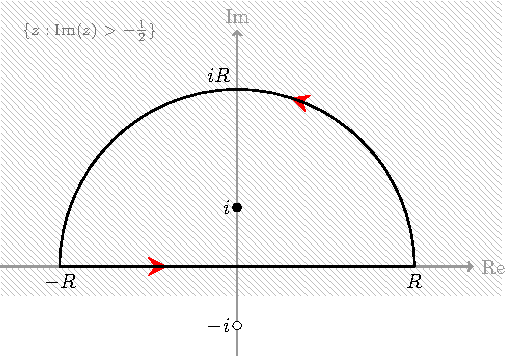
\includegraphics[scale=0.75]{semicircle9}
\end{wrapfigure} 
Previously, we used contour integration to evaluate the (real) integral
\[
\int_{-\infty}^{+\infty} \frac{1}{x^2+1}\ dx,
\]
by considering (the limit as $R \to \infty$ of) the contour integrals
\[
\int_{\mathcal{C}_R} \frac{1}{z^2+1}\ dz,
\]
where $\mathcal{C_R} = L_R+S_R$, with
\begin{itemize}
\item[(i)] $L_R$ the line segment $[-R,R]$ and
\item[(ii)] $S_R$ the semicircular arc, centre 0, radius $R$, joining $R$ to $iR$ through $iR$.
\end{itemize} 

We used the fact that $f$ was holomorphic on a  $\mathcal{R} \backslash \set{i}$, where $\mathcal{R}$ simply connected region containing $\mathcal{C}_R$, together with a factorisation of $f$, in order to apply Cauchy's Integral Formula.
\end{note}

\begin{frame}

\begin{example}
\label{e:gdef}
We shall attempt to evaluate the integral
\[
\int_{\mathcal{C}_R} \frac{1}{z^4+1}\ dz,
\]
\end{example}
where $\mathcal{C}_R=L_R+S_R$ with $R>1$ and
\begin{enumerate}
\item[(i)] $L_R=[-R,R]$, paramterised by $\gamma:[-R,R] \to \C$, $\gamma (t)=t$, 
\item[(ii)] $S_R$ the semicircle parameterised by $\gamma_S:[0,\pi] \to \C$, $\gamma_S (t)=Re^{it}$,
\end{enumerate}
\begin{comment}
Then we have
\[
\int_{\mathcal{C}_R} f = \int_{L_R} f + \int_{S_R} f.
\]
\end{comment}
\end{frame}
\begin{wrapfigure}{r}[2cm]{0.4\textwidth}
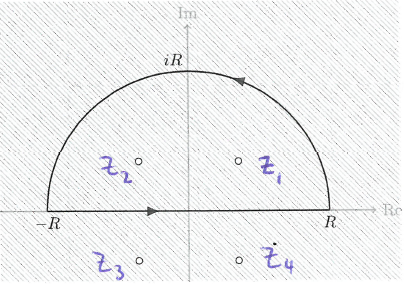
\includegraphics[scale=0.45]{semicircle2a_full}
\end{wrapfigure}The function $f$ is holomorphic on $\C$ except at the points where $z^4+1=0$.  These are the points
\[
z_1=e^{i\pi/4},\ z_2=e^{3i\pi/4},\ z_3=e^{5i\pi/4},\ z_4=e^{7i\pi/4}.
\]
This time, there are \emph{two} points enclosed by $\mathcal{C}_R$ at which $f$ is not holomorphic, and so it is not possible to write
\[
f(z)=\frac{g(z)}{z-z_0}
\]
with $g$ holomorphic on a suitable region $\mathcal{R}$ and $z_0$ a point enclosed by $\mathcal{C}_R$.


If we join $L_R$ and $S_R$ using the line segment $[0,iR]$, we get two simple, closed anticlockwise contours $S^{(1)}$ and $S^{(2)}$ as shown.  Note that each of these contours enclose a single point at which $f$ is not holomorphic.
%\vspace*{3cm}
\begin{figure}[H]
\centerline{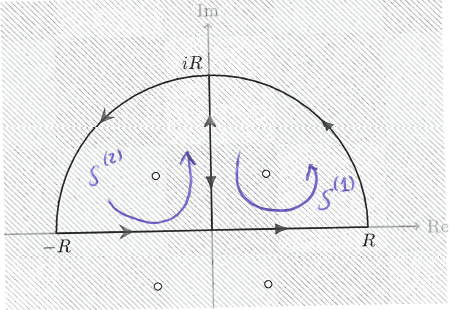
\includegraphics[scale=0.5]{semicircle3_full}}%\quad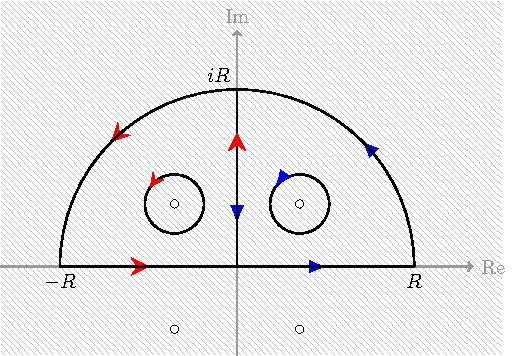
\includegraphics{semicircle4}}
\end{figure}
Since 
\[
\int_{[0,iR]} f = - \int_{[iR,0]} f,
\]
the integral along $[0,iR]$ cancels with the integral along $[iR,0]$ and we get
\[
\int_{S^{(1)}} f + \int_{S^{(2)}} f = \int_{\mathcal{C}_R} f.
\]
%\vspace*{3cm}

Now, if we apply the Shrinking Contour Theorem~\ref{t:sc} to each of $\int_{S^{1}} f$ and $\int_{S^{(2)}} f$, we can replace $S^{(1)}$ and $S^{(2)}$ with small anticlockwise circular contours $C_1$ and $C_2$ around $z_1$ and $z_2$ respectively, so that
\[
\int_{C_1} f = \int_{S^{(1)}} f \quad \text{ and }\quad \int_{C_2} f = \int_{S^{(2)}} f.
\]
\begin{figure}[H]
\centering
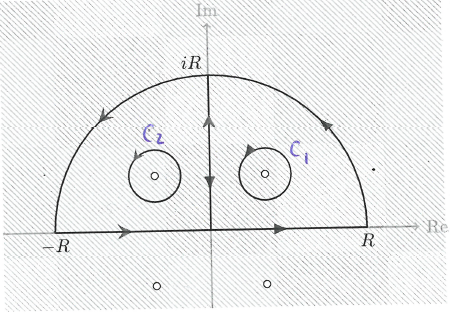
\includegraphics[scale=0.5]{semicircle4_full}
\end{figure}
%\vspace*{3cm}
From here, we may apply Cauchy's Integral Formula (twice) to evaluate
\[
\int_{\mathcal{C}_R} f = \int_{C_1} f + \int_{C_2} f.
\]

\begin{comment}
\begin{example}
Let us use a similar approach to try to evaluate the integral
\[
\int_{-\infty}^{\infty} \frac{1}{(x^2+4)(x^2+9)}\ dx.
\]
\end{example}
This time, we use the same contour $\mathcal{C}_R = L_R+S_R$ and the function
\[
f(z) = \frac{1}{(z^2+4)(z^2+9)}
\]
which is holomorphic on $\C \backslash \set{ \pm 2i,\pm 3i }$ (thus we need to take $R>3$).
\begin{center}
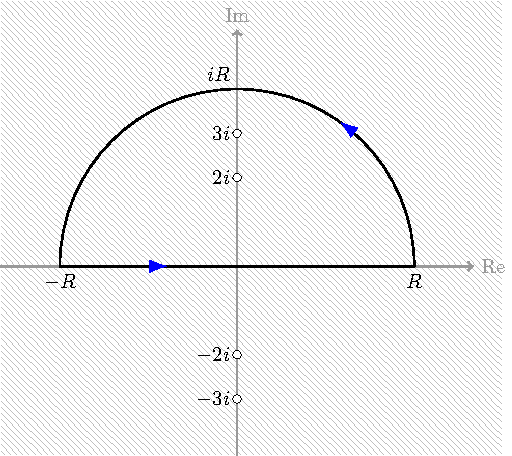
\includegraphics[scale=1]{semicircle5}\\
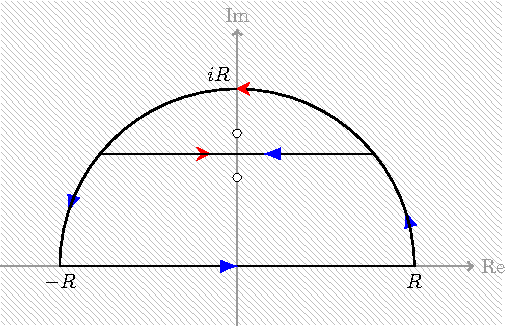
\includegraphics[scale=1]{semicircle6} \\
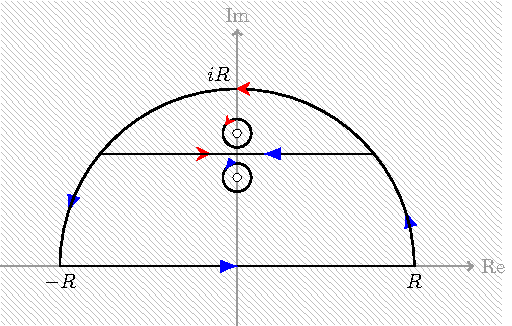
\includegraphics[scale=1]{semicircle7}
\end{center}
\end{comment}

We shall assume that this approach will extend to the case where there is any finite number of points $\set{z_1,z_2,\ldots,z_n}$ enclosed by $\mathcal{C}$ at which $f$ is not holomorphic.
\begin{theorem}[Generalised Shrinking Contour/ Deformation Theorem]
\label{t:gdef}
Let $\mathcal{R}$ be a simply connected region, $\mathcal{C}$ a simple, closed anticlockwise contour in $\mathcal{R}$, and $z_1,z_2,\ldots,z_n$ a finite collection of points that are enclosed by $\mathcal{C}$.  If $f$ is holomorphic on $\mathcal{R} \backslash \set{z_1,\ldots,z_n}$, then 
\[
\int_{\mathcal{C}} f = \int_{\mathcal{C}_1}f+ \ldots + \int_{\mathcal{C}_n} f,
\]
where each $\mathcal{C}_j$ is a closed simple anticlockwise circular contour enclosing $z_j$ and no other $z_k$.
\end{theorem}

\begin{figure}[H]
\centering
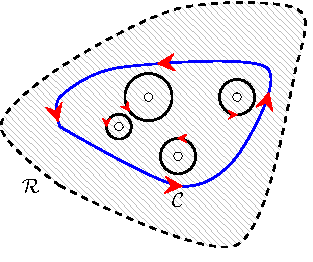
\includegraphics[scale=1]{residues2}
\caption{A contour $\mathcal{C}$ enclosing points $z_1,z_2,z_3$ and $z_4$ at which $f$ is not holomorphic.  The integral of $f$ along $\mathcal{C}$ is determined by the integrals along the circular contours enclosing these points.}
\end{figure}

 Theorem~\ref{t:gdef} allows us, as least in principle, to evaluate each $\int_{\mathcal{C}_j} f$ separately to obtain $\int_{\mathcal{C}} f$.  Thus we have essentially reduced the problem to that of evaluating integrals where there is one point enclosed by the given contour at which $f$ is not holomorphic.  
 
  Sometimes, we will be able to use Cauchy's Integral formula to do this (for example, we could complete Example~\ref{e:gdef} in this way).  This approach will not always work, however.

\begin{example}
\label{e:nonsimplepole}
Let $\mathcal{C}$ be the anticlockwise unit circle and consider the contour integral
\[
\int_{\mathcal{C}} \frac{\sin (z)}{z^2}\ dz.
\]
We cannot write
\[
\frac{\sin (z)}{z^2} = \frac{g(z)}{(z-z_0)}
\]
for any $z_0$ enclosed by $\mathcal{C}$ and $g$ holomorphic on a simply connected region containing $\mathcal{C}$.
\end{example}

In fact, the behaviour encountered in Example~\ref{e:nonsimplepole} will arise whenever we are trying to integrate a function of the form
\[
f(z) = \frac{g(z)}{(z-z_0)^n} \quad (n \geq 2),
\]
where $g$ is holomorphic, $g(z_0) \neq 0$ and $z_0$ is enclosed by $\mathcal{C}$.
\section{Singulairities of complex functions}
Theorem~\ref{t:gdef} shows that when calculating the integral of $f$ along a simple, anticlockwise, closed contour $\mathcal{C}$, the value $\int_{\mathcal{C}} f$ is in some sense depends only on those points at which $f$ is not holomorphic.  Therefore, we shall study these points in more detail.

\begin{definition}
A function $f$ has an \emph{isolated singularity} at the point $z_0$ if for some $r>0$, $f$ is holomorphic on a punctured disc $D'(z_0,r)$ but not on the (unpunctured) open disc $D(z_0,r)$.
\end{definition}
Note that if $f$ has an isolated singularity at $z_0$, it may be the case that $f$ is not defined at $z_0$, or $f$ is defined at $z_0$ but not differentiable there.

\begin{example}
The function $f$ defined by
\[
f(z) = \frac{1}{z^4+1}
\]
has isolated singularities at the points $e^{i\pi/4},\ e^{3i\pi/4},\ e^{5i\pi/4},\ e^{7i\pi/4}$; in each case, take $r = \frac{1}{4}$ for example.
\begin{center}
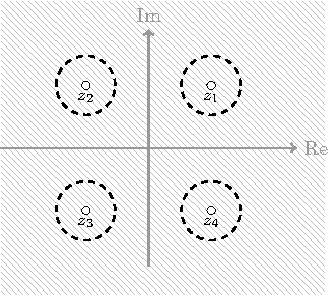
\includegraphics[scale=1]{poles1}
\end{center}
%\vspace*{2cm}

\end{example}
\begin{example}
The function $f$ defined by
\[
f(z) = \frac{\sin (z)}{z^2}
\]
has an isolated singularity at $0$.
\end{example}
\begin{example}
The Principal Logarithm function $\Log : \C \backslash \set{0}$ defined by
\[
\Log (z) = \log(\abs{z}) + i \Arg (z),
\]
is not holomorphic at any point on the negative real axis.  No such point is an isolated singularity of $\Log$
\begin{center}
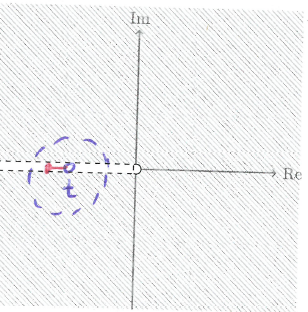
\includegraphics[scale=0.5]{non_iso_full}
\end{center}
Indeed, if $t \leq 0$ is a point on the negative real axis and $r>0$, then $D'(t,r)$ contains points at which $\Log$ is nor holomorphic; $z=t-\frac{r}{2}$ for example.
%\vspace*{3cm}
\end{example}
\begin{definition}  
Let $f$ be continuous on $\mathcal{R} \backslash \set{z_0}$. We say that $\displaystyle \lim_{z \to z_0} f(z) = \infty$ if given any $M>0$ there is some $r>0$ such that
\[
\abs{f(z)}>M \text{ for all } z \in D'(z_0,r).
\]
\end{definition}
\begin{example}

Consider the function
\[
f(z) = \frac{1}{(z-2i)^3}
\]
which has an isolated singularity at $2i$.  We will show that $\displaystyle \lim_{z \to 2i} f(z) = \infty$.

Indeed, given $M>0$, let $r=M^{-1/3}$.  Then 
\begin{align*}
0 < \abs{z-2i} < r \Rightarrow \abs{f(z)} &= \abs{\frac{1}{(z-2i)^3}}\\
& = \frac{1}{\abs{z-2i}^3} \\
& > \frac{1}{(M^{-1/3})^3} = M.
\end{align*}
\end{example}
In most of the examples that we consider, $\displaystyle \lim_{z \to z_0} f(z) = \infty$ will occur whenever evaluating $f$ at $z_0$ would involve division by $0$ (except when $\frac{0}{0}$ would appear).  We shall make this more precise shortly.

\begin{definition}
A function $f$ with an isolated singularity $z_0$ is said to have a \emph{pole at $z_0$} if
\[
\lim_{z \to z_0} f(z) = \infty.
\]
Moreover, for $n \geq 1$, $f$ is said to have a \emph{pole of order $n$} at $z_0$ if for some $r>0$, $f$ can be represented in the form
\[
f(z) = \frac{g(z)}{(z-z_0)^n}\quad\text{ for all } z \in D'(z_0,r)
\]
where $g$ is holomorphic on $D(z_0,r)$ and $g(z_0) \neq 0$.
\end{definition}
Note that the representation
\[
f(z) = \frac{g(z)}{(z-z_0)^n}
\]
need not be valid everywhere on the domain of $f$, only inside the `small' disc $D(z_0,r)$.  The function $g$, unlike $f$, is both defined and differentiable at $z_0$.

\begin{example}
Let us return to the example of
\[
f(z) = \frac{1}{1+z^4}
\]
and investigate the pole $z_1 = e^{i\pi/4}$ of $f$.

Denote by $z_2,z_3$ and $z_4$ the other complex $4^{th}$ roots of $-1$, and let $g$ be the function defined by
\[
g(z) = \frac{1}{(z-z_2)(z-z_3)(z-z_4)}.
\]
Then $g$ is holomorphic on $\C \backslash \set{z_2,z_3,z_4}$, and in particular, holomorphic on $D(z_1,\frac{1}{2})$ for example (the precise value of $r>0$ is not important).
\begin{center}
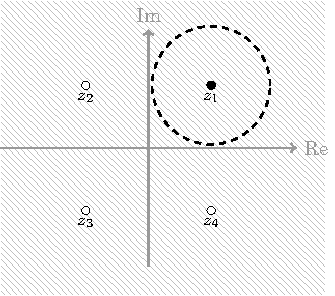
\includegraphics[scale=1]{poles2}
\end{center}
Moreover, $g(z_1) \neq 0$ and
\[
f(z) = \frac{g(z)}{z-z_1} \quad \text{ for all }\quad z \in D'(z_1,\tfrac{1}{2}).
\]
This shows that $f$ has a pole of order $1$ at $z_1$.
\end{example}





%\vspace*{5cm}



\begin{example}
\label{e:poles2}
Let us investigate the poles of  the function
\[
f(z) = \frac{1}{(z^2+9)^2}.
\]
%\vspace*{12cm}
Using the factorisation
\[
z^2+9 = (z+3i)(z-3i)
\]
we have
\[
f(z)= \frac{1}{(z+3i)^2(z-3i)^2}
\]
so that $f$ has isolated singularities at $\pm 3i$.

If we define the function $g_1$ by
\[
g_1(z) = \frac{1}{(z+3i)^2}
\]
then $g_1$ is holomorphic on $\C \backslash \set{-3i}$ and in particular, holomorphic at $3i$ (that is, holomorphic on some open disc centred at $3i$, for example, $D(3i,1)$).  Since
\[
g_1(3i) = - \frac{1}{36} \neq 0 \quad\text{ and }\quad f(z) = \frac{g_1(z)}{(z-3i)^2} \quad\text{ for } z \in D'(3i,1)
\]
we see that $f$ has a pole of order $2$ at $z=3i$.

Similarly, by considering the function $g_2$ defined by
\[
g_2(z) = \frac{1}{(z-3i)^2}
\]
we see that $g_2$ is holomorphic and nonzero at $z=-3i$ and
\[
f(z) = \frac{g_2(z)}{(z+3i)^2}\quad\text{ for }\quad z \in D'(-3i,1)
\]
so that $f$ has a pole of order $2$ at $z=-3i$ also.
\end{example}

%\newpage
\section{The Residue Theorem}

\begin{definition}
Let $f$ have an isolated singularity at $z_0$, then we define the \emph{residue of $f$ at $z_0$}, denoted by $\Res (f;z_0)$, to be
\[
\Res (f;z_0) = \frac{1}{2\pi i} \int_{\mathcal{C}} f
\]
where $\mathcal{C}$ is an anticlockwise simple closed contour which contains $z_0$ and no other singularities of $f$, and lies inside a region in which $f$ is holomorphic.
\end{definition}
If $f$ has an isolated singularity at $z_0$, then such a contour $\mathcal{C}$ can always be found.  Indeed, we know that $f$ is holomorphic on the punctured disc $D'(z_0,r)$ for some $r>0$.  Thus we may take $\mathcal{C}$ to be the anticlockwise circle with centre $z_0$ and radius $r/2$.


For example, we have seen before that with $\mathcal{C}$ the anticlockwise unit circle,
\[
\int_{\mathcal{C}} \frac{1}{z}\ dz=2\pi i \quad \text{ and} \quad \int_{\mathcal{C}} \frac{1}{z^2}\ dz = 0.
\]
Thus for the functions $f$ and $g$ defined by $f(z)=\dfrac{1}{z}$ and $g(z) = \dfrac{1}{z^2}$ we have
\[
\Res (f;0)=1 \quad \text{ and } \quad \Res (g;0) = 0.
\]
%\vspace*{7cm}


Note that Cauchy's Integral Formula may be restated using the language of residues.  Indeed, if
\[
f(z) = \frac{g(z)}{z-z_0}
\]
with $g$ holomorphic on a simply connected region containing $\mathcal{C}$, then $f$ has an isolated singularity at $z_0$ and so
\[
 \Res (f;z_0) = g(z_0)
\]
 
Theorem~\ref{t:residue} is essentially a reformulation of the Generalised Deformation Theorem (Theorem~\ref{t:gdef}).
\begin{theorem}[The Residue Theorem]
\label{t:residue}
Let $\mathcal{R}$ be a simply connected region and let $f$ be a function that is holomorphic on the region $\mathcal{R} \backslash \set{ z_1,z_2,\ldots , z_n}$ and has isolated singularities at the points $z_1,z_2,\ldots,z_n$. If $\mathcal{C}$ is an anticlockwise simple closed contour that lies in $\mathcal{R}\backslash \set{z_1,z_2,\ldots,z_n}$ and encloses the points $z_1,z_2,\ldots,z_n$, then
\[
\int_{\mathcal{C}} f = 2 \pi i \left( \Res (f;z_1)+\Res (f;z_2) + \ldots + \Res (f;z_n ) \right).
\]
\end{theorem}
In other words
\[
\int_{\mathcal{C}} f = 2\pi i \left( \text{ sum of residues of $f$ at isolated singularities enclosed by $\mathcal{C}$ } \right)
\]

\begin{figure}[H]
\centering
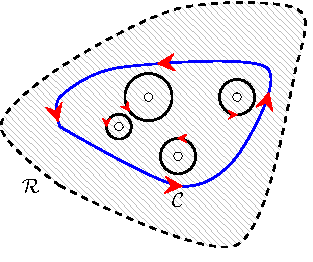
\includegraphics[scale=1]{residues2}
\caption{At each singularity $z_j$, the residue of $f$ at $z_j$ is given by the the integral of $f$ along the small circular contour surrounding $z_j$ (divided by $2\pi i$).  The integral of $f$ along $\mathcal{C}$ is then determined by these residues.}
\end{figure}

We want to use the Residue Theorem to evaluate contour integrals.  The theorem may not look particularly useful yet, since residues themselves are defined to be integrals along circular contours.  However, the following two theorems show us that certain residues may be calculated without performing any integration.



\begin{comment}
\begin{theorem}[Assumption A]
\label{t:assa}
Let $f$ be holomorphic on a region $\mathcal{R}$ and let $z, w \in \mathcal{R}$.  Then
\[
f(z) = f(w) + (z-w) f'(w) + \frac{(z-w)^2}{2!} f''(w) + \ldots + \frac{(z-w)^n}{n!}f^{(n)}(w) + (z-w)^{(n+1)} f_{n+1} (z),
\]
where the function $f_{n+1}$ is holomorphic on $\mathcal{R}$.
\end{theorem}
We make a few observations about Assumption A:
\begin{enumerate}
\item[(i)] Part of Assumption A is the assumption that all derivatives of $f$ exist at $w$.
\item[(ii)] The last term of this sum is $(z-w)^{n+1} f_{n+1} (z)$, and \emph{not} $(z-w)^{n+1} f_{n+1}(w)$.
\item[(iii)] The name $f_{n+1}$ is chosen for convenience - it highlights that the final term depends on our choice of $n$.
\item[(iv)] The assumption is an equality, not an approximation.
\end{enumerate}
\end{comment}

We will need the following Lemma, the proof of which is omitted.
\begin{lemma}
\label{l:goverh}
Suppose that $z_0 \in \C$, $h$ is holomorphic at the point $z_0$ with $h(z_0)=0$ and $h'(z_0) \neq 0$.  Then there is some $\delta>0$ and a holomophic function $k:D(z_0,\delta) \to \C$ with $k(z) \neq 0$ and $h(z)=(z-z_0)k(z)$ for all $z \in D(z_0,\delta)$.
\end{lemma}
\begin{theorem}[The $g/h$ rule]
\label{t:goverh}
Let $z_0 \in \C,\ r>0$ and let $f$ be holomorphic on $D'(z_0,r)$. Suppose that $f$ can be represented by
\[
f(z) = \frac{g(z)}{h(z)}\quad \text{ for } z \in D'(z_0,r)
\]
where $g$ and $h$ are holomorphic on $D(z_0,r)$, and $g(z_0) \neq 0$, $h(z_0)=0$ and $h'(z_0) \neq 0$. Then
\begin{enumerate}
\item[(i)] The function $f$ has an isolated singularity, and in particular, a  pole of order one at $z_0$.
\item[(iii)] The residue of $f$ at $z_0$ is given by
\[
\Res (f,z_0) = \frac{g(z_0)}{h'(z_0)}.
\]
\end{enumerate}
\end{theorem}
\begin{proof}
By Lemma~\ref{l:goverh} we obtain $\delta>0$ (making $\delta<r$ if necessary) and $k:D(z_0,\delta)\to \C$, with $k$ holomorphic and nonzero on $D(z_0,\delta)$ and
\[
f(z)= \frac{g(z)}{k(z)}\cdot \frac{1}{(z-z_0)} \quad \text{ for all } z \in D'(z_0,\delta).
\]
Since $k(z) \neq 0$ for all $z \in D(z_0,\delta)$ the function $z \mapsto \frac{g(z)}{k(z)}$ is holomorphic on $D(z_0,\delta)$, and since $g(z_0) \neq 0$, $f$ has a pole of order $1$ at $z_0$.

If $\mathcal{C}$ is the anticlockwise circle with centre $z_0$ and radius $r/2$, then Cauchy's Integral Formula gives
\[
\Res (f;z_0) = \frac{1}{2\pi i} \int_{\mathcal{C}} f = \frac{1}{2\pi i} \int_{\mathcal{C}} \frac{g(z)}{k(z)} \cdot \frac{1}{z-z_0}\ dz = \frac{g(z_0)}{k(z_0)}.
\]
But then by the product rule, $h'(z) = k(z)+(z-z_0)k'(z)$ for all $z \in D(z_0,\delta)$, so that $h'(z_0) = k(z_0)$, thus
\[
\Res (f;z_0) = \frac{g(z_0)}{h'(z_0)}.
\]
\end{proof}


\begin{comment}
A particularly helpful consequence of Theorem~\ref{t:gh} is as follows: if
\[
f(z) = \frac{g(z)}{z-z_0}
\]
for some function $g$ with $g(z_0) \neq 0$ and $g$ and $g$ holomorphic at $z_0$ (i.e., holomorphic on an open disc containing $z_0$), then
\[
\Res (f;z_0) = g(z_0).
\]
\end{comment}
\begin{example}
Let us calculate the residues at the poles of the function $f$ defined by
\[
f(z) = \frac{1}{1+z^2}.
\]
%\vspace*{12cm}
With $g(z)=1$ and $h(z)=1+z^2$, we have $h(z)=0$ at $z=\pm i$, and $h'(z)=2z \neq 0$ at these points.
Hence $f$ has poles of order $1$ at $z=\pm 1$, with residues
\begin{align*}
\Res (f;i ) & = \frac{g(i)}{h'(i)} = \frac{1}{2i} = - \frac{i}{2} \\
\Res (f;-i) & = \frac{g(-i)}{h'(-i)} = \frac{1}{-2i} = \frac{i}{2}.
\end{align*}

Consider the simple, closed anticlockwise contours $\mathcal{C}_1,\mathcal{C}_2$ and $\mathcal{C}_3$ shown below.
\begin{center}
\hspace*{-2.5cm}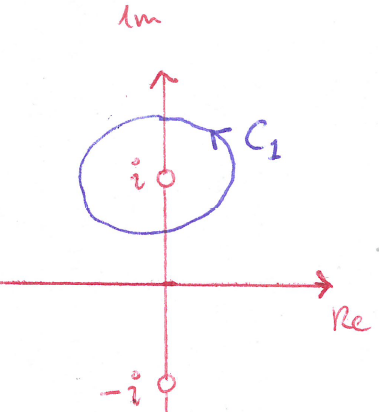
\includegraphics[scale=0.45]{res1full}\ 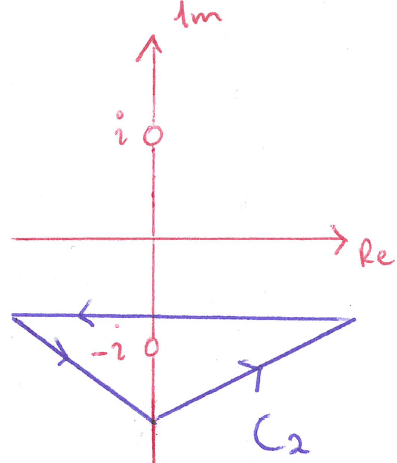
\includegraphics[scale=0.45]{res2full}\ 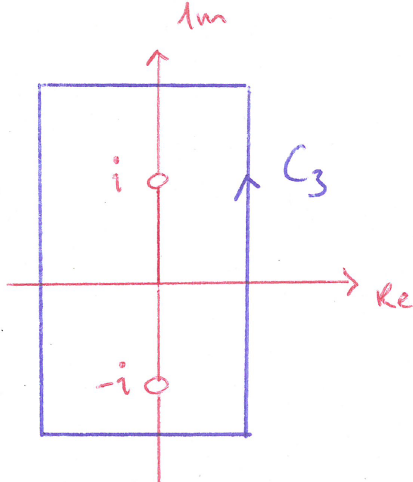
\includegraphics[scale=0.45]{res3full}
\end{center}
By the Residue Theorem, we have
\begin{align*}
\int_{\mathcal{C}_1} f &= 2\pi i \left[ \Res (f;i) \right] = 2\pi i \left[ \frac{-i}{2} \right] = \pi \\
\int_{\mathcal{C}_2} f &= 2\pi i \left[ \Res (f;-i) \right] =2\pi i \left[ \frac{i}{2} \right] = -\pi\\
\int_{\mathcal{C}_3} f &= 2\pi i \left[ \Res (f;i)+\Res(f;-i) \right] = 2\pi i \left[ -\frac{i}{2} + \frac{i}{2} \right] = 0,
\end{align*}
since $\mathcal{C}_1$ encloses the singularity $z=i$ and no others, $\mathcal{C}_2$ encloses the singularity $z=-i$ and no others, and $\mathcal{C}_3$ encloses the singularities $z=i$ and $z=-i$.
\end{example}
\begin{example}
Let us do the same for the function
\[
f(z) = \frac{-i}{6z^2+13z+6}
\]
Let $g(z)=-i$ and 
\[
h(z) = 6z^2+13z+6 = (3z+2)(2z+3)
\]
and note that $h(z)=0$ for $z=-\frac{2}{3},-\frac{3}{2}$.  Since $h'(z)=12z+13$, we have
\[
h'(-2/3)  = 5 \quad\text{ and}\quad h'(-3/2) = -5,
\]
both of which are nonzero, so that $f$ has poles of order $1$ at $-\frac{2}{3}$ and $-\frac{3}{2}$ by Theorem~\ref{t:goverh}.  Moreover, by the same result,
\begin{align*}
\Res(f;-2/3) & = \frac{g(-2/3)}{h'(-2/3)} = - \frac{i}{5} \\
\Res (f;-3/2) & = \frac{g(-3/2)}{h'(-3/2)} = \frac{i}{5}.
\end{align*}
Note that if $\mathcal{C}$ is the anticlockwise unit circle, then only the poles $z=-2/3$ is enclosed by $\mathcal{C}$, so that by the Residue Theorem
\[
\int_{\mathcal{C}} f = 2\pi i \left( \frac{-i}{5} \right) = \frac{2\pi}{5}
\]
(compare Example~\ref{e:trig1}).
\end{example}
%\vspace*{20cm}
%\begin{absolutelynopagebreak}
\begin{theorem}
\label{t:polen}
Let $f$ have an isolated singularity at $z_0$ which is a pole of order $n$, so that for some $r>0$
\[
f(z) = \frac{g(z)}{(z-z_0)^n} \quad \text{ for } z \in D'(z_0,r),
\]
with $g$ holomorphic on $D(z_0,r)$ and $g(z_0) \neq 0$.  Then
\[
\Res (f,z_0) = \frac{g^{(n-1)}(z_0)}{(n-1)!}.
\]
\end{theorem}
%\end{absolutelynopagebreak}
%\noindent\textit{Proof:}
\begin{proof}
By definition,
\[
\Res (f;z_0) = \frac{1}{2\pi i} \int_{\mathcal{C}} \frac{g(z)}{(z-z_0)^n}\ dz,
\]
where $\mathcal{C}$ is the anticlockwise circle with centre $z_0$ and radius $r/2$.  By Theorem~\ref{t:cauchyd} (Cauchy's Integral Formula for Derivatives),
\[
g^{(n-1)} (z_0) = \frac{(n-1)!}{2\pi i} \int_{\mathcal{C}} \frac{g(z)}{(z-z_0)^n}\ dz,
\]
so that
\[
g^{(n-1)} (z_0) = (n-1)!\ \Res (f;z_0),
\]
or in other words,
\[
\Res (f;z_0) = \frac{g^{(n-1)}(z_0)}{(n-1)!}.
\]
\end{proof}
%\vspace*{10cm}



\begin{example}
\label{e:res3}
%\begin{absolutelynopagebreak}
Let us consider the function $f$ defined by
\[
f(z) = \frac{1}{(z^2+9)^2}.
\]
and calculate the residues at the poles of $f$.
%\end{absolutelynopagebreak}
Following Example~\ref{e:poles2}, we define $g_1$ and $g_2$ by
\[
g_1(z) = \frac{1}{(z+3i)^2} \quad\text{ and }\quad g_2(z) = \frac{1}{(z-3i)^2}
\]
so that
\[
f(z) = \frac{g_1(z)}{(z-3i)^2} = \frac{g_2(z)}{(z+3i)^2},
\]
and $g_1$ is holomorphic and nonzero at $z=3i$, $g_2$ is holomorphic and nonzero at $z=-3i$.  

Since the poles at $z=\pm 3i$ both have order $2$, Theorem~\ref{t:polen} tells us that
\[
\Res (f;3i) =\frac{g_1'(3i)}{1!} \quad\text{ and } \Res (f;-3i) = \frac{g_2'(-3i)}{1!}.
\]
The required derivatives are
\begin{align*}
g_1'(z) = -2(z+3i)^{-3} & \Rightarrow g_1'(3i) = -2(3i+3i)^{-3} = - \frac{i}{108} \\
g_2'(z) = -2(z-3i)^{-3} & \Rightarrow g_2'(-3i) = -2(-3i-3i)^{-3} = \frac{i}{108},
\end{align*}
Hence
\[
\Res (f;3i) = \frac{-i/108}{1!} = - \frac{i}{108} \quad\text{ and }\quad \Res (f;-3i) = \frac{i/108}{1!}= \frac{i}{108}.
\]
%\vspace*{15cm}

\end{example}

\begin{example}
%\begin{absolutelynopagebreak}
For the function $f$ defined by
\[
f(z) = \frac{\exp(\pi z)}{(z-i)^3}
\]
find $\Res (f,i)$.  Hence evaluate
\[
\int_{\mathcal{C}} \frac{\exp( \pi z)}{(z-i)^3}\ dz,
\]
where $\mathcal{C}$ is the anticlockwise triangular contour with vertices $2$, $2i$ and $-2$.
%\end{absolutelynopagebreak}
%\vspace*{15cm}

The only pole of $f$ is a pole of order $3$ at $z=i$.  With $g$ the holomorphic function defined by $g(z) = \exp(\pi z )$, we have $g'(z) = \pi \exp(\pi z)$ and $g''(z) = \pi^2 \exp(\pi z)$.  By Theorem~\ref{t:polen},
\[
\Res(f;i) = \frac{g''(i)}{2!} = \frac{\pi^2 \exp(\pi i)}{2!} = \frac{\pi^2(-1)}{2} = - \frac{\pi^2}{2}.
\]
Since $\mathcal{C}$ is a simple, closed anticlcokwise contour, and $i$ is the only pole of $f$ enclosed by $\mathcal{C}$, the Residue Theorem gives
\[
\int_{\mathcal{C}} f = 2\pi i \Res (f;i) = 2\pi i \left( -\frac{\pi^2}{2} \right) = -i \pi^3.
\]
\end{example}

%\newpage
\section{Evaluating Real Integrals using Contour Integration, part 2}
\begin{example}
Let us evaluate
\[
\int_{-\infty}^{+\infty} \frac{1}{(x^2+9)^2}\ dx
\]
using contour integration.

We shall follow the approach used in Example~\ref{e:realint1}, by considering the complex function $f$ defined via
\[
f(z) = \frac{1}{(z^2+9)^2}
\]
and the contour $\mathcal{C}_R=L_R+S_R$, where $R>3$, $L_R=[-R,R]$ and $S_R$ is the upper semicircle with centre $0$ and radius $R$ from $R$ to $-R$ via $iR$.

Using the result of Example~\ref{e:res3}, the only singularity of $f$ enclosed by $\mathcal{C}_R$ is at $z=3i$, hence by the Residue Theorem
\[
\int_{\mathcal{C}_R} f = 2\pi i \Res (f;3i) = 2\pi i \left( -\frac{i}{108} \right) = \frac{\pi}{54}
\]
for all $R>3$.

If $z \in S_R$, then $\abs{z}=R$ and hence by the reverse triangle inequality
\[
\abs{z^2+9} \geq \abs{\abs{z^2}-9} = \abs{\abs{z}^2-9} = R^2-9,
\]
so that for all such $z$ we have $\abs{z^2+9}^2 \geq \left( R^2-9 \right)^2$.  Thus for all $z \in S_R$,
\[
\abs{\frac{1}{(z^2+9)^2}} = \frac{1}{\abs{z^2+9}^2} \leq \frac{1}{\left(R^2-9 \right)^2}.
\]
The Estimation Lemma gives
\[
\abs{ \int_{\mathcal{C}_R} \frac{1}{(z^2+9)^2}\ dz } \leq \frac{1}{\left(R^2-9 \right)^2} \cdot \pi R,
\]
hence $\displaystyle \int_{\mathcal{C}_R} f \to 0$ as $R \to \infty$ as before.

Parameterising $L_R$ using $\gamma:[-R,R] \to \C$, $\gamma(t)=t$ we have $\gamma'(t)=1$ and so
\[
\int_{L_R} f = \int_{-R}^{R} \frac{1}{(t^2+9)^2}\ dt.
\]
Hence
\begin{align*}
\frac{\pi}{54} & = \int_{\mathcal{C}_R} f  && (\forall\ R>3) \\
& = \lim_{R \to \infty} \int_{\mathcal{C}_R} f && \\
& = \lim_{R \to \infty} \left( \int_{L_R} f \right) + \lim_{R \to \infty} \left( \int_{S_R} f \right) && \\
& = \lim_{R \to \infty} \int_{-R}^{+R} \frac{1}{(t^2+9)^2}\ dt\ +0&& \\
 &= \int_{-\infty}^{+\infty} \frac{1}{(t^2+9)^2}\ dt. &&
\end{align*}
(Note that it does not matter whether we call the variable of integration $x$ or $t$).
\end{example}
%\vspace*{20cm}

%\newpage
%\vspace*{5cm}
%\newpage
\begin{example}
Evaluate
\[
I = \int_0^{\infty} \frac{\cos(x)}{x^4+1}\ dx.
\]
using contour integration.
\end{example}
\begin{enumerate}
\item Since both $x \mapsto \cos (x)$ and $x \mapsto x^4$ are even functions of $x$, we have
\[
I = \frac{1}{2} \int_{-\infty}^{+\infty} \frac{\cos(x)}{x^4+1}\ dx.
\]
\item To evaluate this integral, we shall integrate a suitable complex function $f$ along the contour $\mathcal{C}_R=L_R+S_R$ as before, and consider the limit as $R \to \infty$.  Our hope is that as $R \to \infty$, we will have $\int_{S_R} f \to 0$, and $\int_{L_R} f$ will give us the value of $I$.

\item We need a suitable complex function.  We could try this using
\[
f(z) = \frac{\cos (z)}{z^4+1}
\]
but since $\cos(z) =\frac{1}{2} (\exp(iz)+\exp(-iz))$, for the point $iR \in S_R$ we have
\[
\cos(iR) = \frac{\exp(iiR)+\exp(-iiR)}{2} = \frac{e^{-R}+e^R}{2},
\]
and $e^R \to \infty$ as $R \to \infty$, which is a problem, as we want $\int_{S_R} f \to 0$.

Instead, we use the fact that
$
\exp (ix) = \cos (x) + i \sin (x)
$ and so $\cos(x) = \Re (\exp(ix))$ for all $x \in \R$. This implies
\[
I = \frac{1}{2} \int_{-\infty}^{\infty} \frac{\Re ( \exp(ix) )}{x^4 +1}\ dx = \frac{1}{2} \Re \left( \int_{-\infty}^{+\infty} \frac{\exp(ix)}{x^4+1}\ dx \right).
\]

Thus we shall consider the complex function
\[
f(z) = \frac{\exp(iz)}{z^4+1}
\]
which is holomorphic everywhere in $\C$ except where $z^4=-1$; that is to say, $f$ is holomorphic on $\C \backslash \set{ e^{i\pi/4},\ e^{i3\pi/4},\ e^{i 5\pi/4},\ e^{i 7\pi/4} }$.
\end{enumerate}
So (for $R>1$) we have
\begin{align*}
\int_{\mathcal{C}_R} f &= 2\pi i \left( \text{ sum of residues at poles of $f$ inside $\mathcal{C}_R$} \right) \\
& = 2\pi i \left( \Res (f;e^{i\pi/4})+\Res(f;e^{3i\pi/4}) \right)
\end{align*}
by the Residue Theorem.
\begin{center}
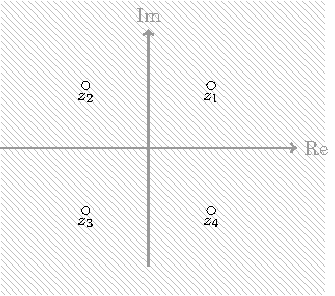
\includegraphics[scale=1]{poles3}
\end{center}
%\vspace*{10cm}
Write
\begin{align*}
e^{i\pi/4} & = \polar{}{\pi/4} && \\
& = \frac{1}{\sqrt{2}} + i \frac{1}{\sqrt{2}} =a+ia && \text{ where } a = \frac{1}{\sqrt{2}}.
\end{align*}
Then
\[
e^{i3\pi/4} = \cos (3\pi/4)+i \sin (3\pi/4) = -\frac{1}{\sqrt{2}}+i \frac{1}{\sqrt{2}} = -a +ia.
\]
Let $g(z) = \exp (iz)$ and $h(z) = z^4+1$ so that $f=g/h$ and $h'(z) = 4z^3$, hence
\begin{align*}
h'(e^{i\pi/4}) &= 4 (e^{i\pi/4})^3 = 4e^{i3\pi/4} = 4(-a+ia) \neq 0 \\
h'(e^{i3\pi/4}) & = 4 (e^{i3\pi/4})^3 = 4e^{9i\pi/4} = 4e^{i\pi/4} = 4 (a+ia) \neq 0.
\end{align*}
Thus by the $g/h$ rule, $f$ has poles of order $1$ at $e^{i\pi/4}$ and $e^{i3\pi/4}$, and the corresponding residues are
\begin{align*}
\Res (f;e^{i\pi/4}) & = \frac{g(e^{i\pi/4})}{h'(e^{i\pi/4})} \\
& = \frac{\exp (i(a+ia))}{4(-a+ia)} \\
& = \frac{\exp(-a+ia)}{4(-a+ia)} \\
& = \frac{e^{-a}}{4a} \cdot \frac{\exp(ia)}{-1+i} \cdot \frac{-1-i}{-1-i} \\
& = \frac{e^{-a}}{4a} \frac{(\cos(a)+i\sin(a))(-1-i)}{(-1)^2+(1)^2} \\
& = \frac{e^{-a}}{8a} \left[ (-\cos(a)+\sin(a))+ i (-\cos(a)-\sin(a)) \right], 
\end{align*}
and
\begin{align*}
\Res (f;e^{i3\pi/4}) & = \frac{g(e^{i3\pi/4})}{h'(e^{i3\pi/4})} \\
& = \frac{\exp(i(-a+ia)}{4(a+ia)} \\
& = \frac{\exp(-a-ia)}{4a(1+i)} \\
& = \frac{e^{-a}}{4a} \cdot \frac{\exp(-ia)}{1+i} \cdot \frac{1-i}{1-i} \\
& = \frac{e^{-a}}{4a} \cdot \frac{(cos(-a)+i \sin(-a))(1-i)}{(1)^2+(1)^2} \\
& = \frac{e^{-a}}{8a} \left[ (\cos(-a) + \sin (-a))+i(-\cos(-a) + \sin(-a) ) \right] \\
& = \frac{e^{-a}}{8a} \left[ ( \cos(a)-\sin(a) ) + i (-\cos(a)-\sin(a)) \right].
\end{align*}

Thus by the Residue Theorem,
\begin{align*}
\int_{\mathcal{C}_R} f & = 2\pi i \left( \Res (f;e^{i\pi/4}) +\Res (f;e^{i3\pi/4}) \right) \\
& = 2 \pi i \left( \frac{e^{-a}}{8a} \left[ (-\cos(a)+\sin(a))+ i (-\cos(a)-\sin(a)) \right] \right. \\ &\ + \left. \frac{e^{-a}}{8a} \left[ ( \cos(a)-\sin(a) ) + i (-\cos(a)-\sin(a)) \right] \right) \\
& = \frac{\pi ie^{-a}}{4a} \left( i (-2\cos(a)-2\sin(a)) \right) \\
& = \frac{\pi  e^{-a}}{2a} \left( \cos(a) + \sin (a) \right) \\
& = \frac{\pi}{\sqrt{2}}\ e^{-1/\sqrt{2}} \left( \cos (1/\sqrt{2}) + \sin (1/\sqrt{2}) \right).
\end{align*}




We have evaluated
\[
\int_{\mathcal{C}_R} f
\]
using contours, now we look at
\[
\int_{\mathcal{C}_R} f = \int_{L_R} f + \int_{S_R} f.
\]
We want to show that as $R \to \infty$,
\[
\int_{S_R} f \to 0 
\]
and that we may deduce the value of $I$ from $\displaystyle \int_{L_R} f$.


First of all, we note that for $z=x+iy \in S_R$, we have 
\begin{align*}
\abs{\exp(iz)} & = \abs{ \exp (-y+ix) } \\
& = \abs{e^{-y} \left( \cos (x) + i \sin (x) \right) } \\
& = \abs{ e^{-y} } \cdot \abs{ \cos(x) + i \sin (x) } \\
& = e^{-y}.
\end{align*}
Since $S_R$ lies above the real axis, we have $y \geq 0$ whenever $z=x+iy \in S_R$, and thus
\[
\abs{\exp(iz) } = e^{-y} \leq 1
\]
for all such $z$.  Moreover, the reverse triangle inequality shows that
\[
\abs{z^4+1} \geq \abs{ \abs{z^4} - \abs{1} } = \abs{ \abs{z}^4-1} = R^4-1
\]
whenever $R>1$.  Hence for $R>1$,
\[
\abs{ f(z) } = \abs{ \frac{\exp(iz)}{z^4+1} } \leq \frac{1}{R^4-1} \quad \text{ for all } z \in S_R.
\]
Together with the Estimation Lemma and the fact that $S_R$ has length $\pi R$, we see that
\[
\abs{ \int_{S_R} f } \leq \frac{1}{R^4-1} \cdot \pi R
\]
for all $R>1$, and so
\[
\int_{S_R} f \to 0 \quad\text{ as }\quad R \to \infty.
\]

Now let us examine the integral $\displaystyle \int_{L_R} f$.  Using the parameterisation $\gamma_L:[-R,R] \to \C$, $\gamma_L (t) = t$, we have $\gamma ' (t) = 1$ and so
\begin{align*}
\int_{L_R} f &= \int_{-R}^R \frac{\exp(it)}{t^4+1}\ dt \\
& = \int_{-R}^{R} \left( \frac{\cos(t)}{t^4+1} + i\ \frac{\sin(t)}{t^4+1} \right)\ dt \\
& = \int_{-R}^R \frac{\cos(t)}{t^4+1}\ dt + i \int_{-R}^R \frac{\sin(t)}{t^4+1}\ dt.
\end{align*}
In other words, for all $R$ we have
\[
\int_{-R}^R \frac{\cos(t)}{t^4+1}\ dt = \Re \left( \int_{L_R} f \right).
\]
Hence
\begin{align*}
\frac{\pi}{\sqrt{2}} e^{-1/\sqrt{2}} \left( \cos (1/\sqrt{2})+\sin(1/\sqrt{2}) \right) & = \int_{C_R} f \\
& = \lim_{R \to \infty} \int_{C_R} f \\
& = \lim_{R \to \infty} \int_{L_R} f + \lim_{R \to \infty} \int_{S_R} f \\
& = \lim_{R \to \infty} \int_{-R}^{R} \frac{\exp(it)}{t^4+1}\ dt \\
& = \lim_{R \to \infty} \int_{-R}^{R} \frac{\cos(t)}{t^4+1}\ dt + i \lim_{R \to \infty} \int_{-R}^R \frac{\sin(t)}{t^4+1}\ dt \\
&=  \int_{-\infty}^{\infty} \frac{\cos(t)}{t^4+1}\ dt + i \int_{-\infty}^{\infty} \frac{\sin (t)}{t^4+1}\ dt.
\end{align*}
Equating the real and imaginary parts of both sides we see that
\[
\int_{-\infty}^{+\infty}  \frac{\cos(t)}{t^4+1}\ dt = \frac{\pi}{\sqrt{2}} e^{-1/\sqrt{2}} \left( \cos (1/\sqrt{2})+\sin(1/\sqrt{2}) \right) \quad\text{ and }\quad \int_{-\infty}^{\infty} \frac{\sin (t)}{t^4+1}\ dt =0.
\]
Hence
\begin{align*}
\int_0^{\infty} \frac{\cos(x)}{x^4+1}\ dx &= \frac{1}{2} \int_{-\infty}^{\infty} \frac{\cos(x)}{x^4+1}\ dx \\
& = \frac{\pi}{2\sqrt{2}} e^{-1/\sqrt{2}} \left( \cos (1/\sqrt{2})+\sin(1/\sqrt{2}) \right).
\end{align*}
The following example is from the 2012 exam paper
\begin{example}
Use contour integration to evaluate
\[
\int_0^{\infty} \frac{\cos(5x)}{x^2+9}\ dx.
\]
[You may use without proof the fact that
\[
\lim_{R \to \infty} \int_{S_R} \frac{\exp(5iz)}{z^2+9}\ dz = 0,
\]
where $S_R$ is the upper semicircle from $R$ to $-R$.]
\end{example}
\begin{solution}
Since the integrand is an even function of $x$, we have
\[
\int_{0}^{\infty} \frac{\cos(5x)}{x^2+9}\ dx = \frac{1}{2} \int_{-\infty}^{\infty} \frac{\cos(5x)}{x^2+9}\ dx.
\]
We shall use the contour $\mathcal{C}_R = L_R+S_R$ as before, where $R>3$, $L_R=[-R,R]$ and $S_R$ is the upper semicircle from $R$ to $-R$ via $iR$.  To find a suitable complex function to integrate, we use the fact that for $x \in R$,
\[
\exp(5ix) = \cos(5x) + i \sin (5x),
\]
so that for all $R>0$,
\[
\int_{-R}^{R} \frac{\cos(5x)}{x^2+9}\ dx = \Re \left(\int_{-R}^R \frac{\exp(5ix)}{x^2+9}\ dx \right).
\]

Thus we shall use the function $f$ defined by
\[
f(z) = \frac{\exp(5iz)}{z^2+9}.
\]
This function has isolated singularities at $z=\pm 3i$, and of these, only $z=3i$ is enclosed by $\mathcal{C}_R$.  With $g(z) = \exp(5iz)$ and $h(z)=z^2+9$, we have $f=g/h$ and $h'(z)=2z$.  Hence by the $g/h$ rule,
\[
\Res (f;3i) = \frac{g(3i)}{h'(3i)} = \frac{\exp(3i)(5i)}{2(3i)} = \frac{e^{-15}}{6i}.
\]
By the Residue Theorem,
\[
\int_{\mathcal{C}_R} f = 2\pi i \left( \frac{e^{-15}}{6i} \right) = \frac{\pi}{3e^{15}}
\]
for all $R>3$.

We are given that 
\[
\int_{S_R} f \to 0 \quad\text{ as}\quad R \to \infty,
\]
and parameterising $L_R$ with the function $\gamma_L:[-R,R] \to \C$, $\gamma(t)=t$, we see that
\[
\int_{L_R} f = \int_{-R}^R \frac{\exp(5it)}{t^2+9}\ dt = \left(\int_{-R}^R \frac{\cos(5t)}{t^2+9}\ dt\right) + i \left( \int_{-R}^R \frac{\sin(5t)}{t^2+9}\ dt \right).
\]
Hence
\begin{align*}
\frac{\pi}{3e^{15}} & = \int_{\mathcal{C}_R} f \\
& = \lim_{R \to \infty} \int_{\mathcal{C}_R} f \\
& = \lim_{R \to \infty} \int_{L_R} f + \lim_{R \to \infty} \int_{S_R} f \\
& = \lim_{R \to \infty} \left( \left(\int_{-R}^R \frac{\cos(5t)}{t^2+9}\ dt\right) + i \left( \int_{-R}^R \frac{\sin(5t)}{t^2+9}\ dt \right) \right) + 0 \\
& = \int_{-\infty}^{\infty} \frac{\cos(5t)}{t^2+9}\ dt + i\ \int_{-\infty}^{\infty} \frac{\sin(5t)}{t^2+9}\ dt.
\end{align*}
Equating the real  parts of both sides, we see that
\[
\frac{\pi}{3e^{15}} = \int_{-\infty}^{\infty} \frac{\cos(5t)}{t^2+9}\ dt
\]
hence
\[
\int_0^{\infty} \frac{\cos(5x)}{x^2+9}\ dt = \frac{\pi}{6e^{15}}.
\]
\end{solution}

The next example is from the 2014 exam.
\begin{example}
Show that
\[
\int_{\mathcal{C}} \left( \frac{z+z^{-1}}{2} \right)^4 \frac{1}{iz}\ dz = \int_0^{2\pi} (\cos(t))^4\ dt
\]
where $\mathcal{C}$ is the anticlockwise contour whose points lie on the circle $\set{z: \abs{z}= 1 }$, and evaluate this integral.

Find the value of the integral
\[
\int_0^{2\pi} \left( (\cos(t))^6+(\sin (t))^6 \right)\ dt.
\]
\end{example}
\begin{solution}
Let us define a function $f$ by
\[
f(z) =\left( \frac{z+z^{-1}}{2} \right)^4 \frac{1}{iz},
\]
and parameterise $\mathcal{C}$ using the function $\gamma:[0,2\pi ] \to \C,\ \gamma(t)=e^{it}$.  Then since $\gamma'(t)=ie^{it}$, the definition/formula
\[
\int_{\mathcal{C}} f = \int_0^{2\pi} f (\gamma (t)) \gamma' (t)\ dt,
\]
gives
\begin{align*}
\int_{\mathcal{C}} \left( \frac{z+z^{-1}}{2} \right)^4 \frac{1}{iz}\ dz & = \int_0^{2\pi} \left( \frac{e^{it}+e^{-it}}{2} \right)^4 \cdot \frac{1}{ie^{it}} \cdot ie^{it}\ dt \\
& = \int_0^{2\pi} \left( \frac{e^{it}+e^{-it}}{2} \right)^4 \ dt \\
& = \int_0^{2\pi} (\cos(t))^4\ dt.
\end{align*}

To evaluate this integral, we first expand $(z+z^{-1})^4$ using the Binomial formula:
\[
(z+z^{-1})^4 = z^4+4z^2+6+4z^{-2}+z^{-4}.
\]
Hence
\[
\left( \frac{z+z^{-1}}{2} \right)^4 \frac{1}{iz} = \frac{1}{16i} \left(z^3+4z+6z^{-1}+4z^{-3}+z^{-5} \right).
\]
Note that all terms of this sum have antiderivatives on $\C \backslash \set{0}$ except for the $z^{-1}$ term.  Hence by the Fundamental Theorem of Calculus,
\[
\int_{\mathcal{C}} f = \int_{\mathcal{C}} \frac{1}{16i} \cdot \frac{6}{z} \ dz = \frac{3}{8i} \int_{\mathcal{C}} \frac{1}{z}\ dz.
\]
By the $g/h$ rule and the Residue Theorem,
\[ \int_{\mathcal{C}} \frac{1}{z}\ dz = 2\pi i,
\]
hence
\[
\int_{\mathcal{C}} f = \frac{3}{8i} \cdot 2\pi i = \frac{3\pi}{4}.
\]

In exactly the same way,
\[
\int_0^{2\pi} \left( \cos (t) \right)^6\ dt = \int_{\mathcal{C}} \left( \frac{z+z^{-1}}{2} \right)^6 \frac{1}{iz}\ dz,
\]
and only the $z^{-1}$ term contributes to this integral.  To find this, we find the constant term of $(z+z^{-1})^6$ using the Binomial Formula:
\[
(z+z^{-1})^6 = z^6 + \ldots + \binom{6}{3} + \ldots + z^{-6}.
\]
Thus
\[
\left( \frac{z+z^{-1}}{2} \right)^6 \frac{1}{iz} = \frac{1}{i2^6} \left( \ldots + \binom{6}{3} z^{-1} + \ldots \right)
\]
so that 
\[
\int_{\mathcal{C}} \left( \frac{z+z^{-1}}{2} \right)^6 \frac{1}{iz}\ dz =  \frac{\binom{6}{3}}{i2^6} \int_{\mathcal{C}} \frac{1}{z}\ dz = \frac{5\pi}{8}.
\]

Doing the same for the sine function:
\begin{align*}
\int_0^{2\pi} \left( \sin (t) \right)^6\ dt &= \int_{\mathcal{C}} \left( \frac{z-z^{-1}}{2i} \right)^6 \frac{1}{iz}\ dz \\
& = \frac{\binom{6}{3}}{(2i)^6} \int_{\mathcal{C}} \frac{1}{z}\ dz \\
& = \frac{5\pi}{8}.
\end{align*}
Hence
\[
\int_0^{2\pi} \left( (\cos(t))^6+(\sin (t))^6 \right)\ dt = \frac{5\pi}{4}.
\]
\end{solution}
\begin{comment}
\section{The Taylor Series of a Holomorphic Function}
\begin{theorem}{Taylor Series}
\label{t:taylor}
Let $w \in \C$, $r>0$ and let $f$ be holomorphic on $D(w,r)$.  Then there exist coefficients $c_1,c_2,\ldots \in \C$ such that
\[
f(z) = \sum_{n=0}^{\infty} c_n (z-w)^n
\]
for all $z \in D(w,r)$.
\end{theorem} 
To say that 
\[
f(z) = \sum_{n=0}^{\infty} c_n (z-w)^n,
\]
we mean that the series on the right hand side converges to $f(z)$.  In other words,
\[
\lim_{n \to \infty} \abs{ f(z) - \sum_{n=0}^{\infty} c_n (z-w)^n} =0
\]
for all $z \in D(w,r)$.  The sums $\displaystyle \sum_{k=0}^n c_k (z-w)^k$ are called the \emph{partial sums} of the series $\displaystyle \sum_{k=0}^{\infty} c_k (z-w)^k$.  The series $\displaystyle \sum_{k=0}^{\infty} c_k (z-w)^k$ itself is called the \emph{Taylor Series (expansion) of $f$ at $w$}, or sometimes the \emph{Power Series} expansion of $f$ at $w$.

We can of course rewrite as
\[
f(w+h) = \sum_{n=0}^{\infty} c_n h^n
\]
whenever $\abs{h} <R$.

\begin{proof}{(of Theorem~\ref{t:taylor})}

\end{proof}
\end{comment}